\documentclass[11pt,a4paper]{article}
\usepackage[utf8]{inputenc}
\usepackage[french]{babel}
\usepackage[T1]{fontenc}
\usepackage{mathtools}
\usepackage{tikz}
\usepackage{amsmath, amssymb, amsthm}            
\usepackage{amstext, amsfonts, a4}
\usepackage{hyperref}
\usepackage[ruled,vlined, french, onelanguage]{algorithm2e}
\usepackage[left=2cm,right=2cm,top=2cm,bottom=2cm]{geometry}
\usepackage{multicol}
\usepackage{xcolor}
\usepackage{float}
\usepackage{lscape}


\begin{document}
\begin{algorithm}[H]
\SetAlgoLined
Soit $A:=\left(\begin{array}{c|c}
M_{\cdot D} & 0\\
\hline
0 & \frac{1}{\Delta t}\text{Id}
\end{array}\right)$\\
~\\
\ForEach{$p_k$ : points du bord}
{
	~\\
	\textbf{$p_k$ : le point de bord considéré, d'indice global $k$}\\
	~\\
	\If{$p_k$ est un point du maillage} 
	{	
		\textcolor{red}{\textbf{On passe au point $p_k$ suivant}}\\
	}
	~\\
	\textbf{$p_l$ : premier voisin de $p_k$, d'indice global $l$}\\
	\textbf{$p_r$ : deuxième voisin de $p_k$, d'indice global $r$}\\
	~\\
	\textbf{$\gamma$ : axe sur lequel est placée l'arête $[p_l,p_r]$ (ie soit $x$ ou $y$ ou $z$)}\\
	~\\
	\textcolor{red}{\textbf{Nous devons dans un premier temps supprimer les interactions entre $p_l$ et $p_r$ :}}
	\begin{center}
	$A [l, r] = A [r, l] = 0$
	\end{center}
	\textcolor{red}{\textbf{Ensuite actualisons la ligne $k$ :}}
	\begin{center}
	$A [k, :] = 0$\hspace{1cm}\textbf{Actualise\_ligne $(k, \gamma)$}
	\end{center}
	\textcolor{red}{\textbf{Enfin actualisons les lignes $l$ et $r$ :}}
	\begin{center}
	\textbf{Actualise\_ligne $(l, \gamma)$}\hspace{1cm}
	\textbf{Actualise\_ligne $(r, \gamma)$}
	\end{center}
}
\caption{Insertion de coefficients dans la matrice}
\end{algorithm}

\begin{algorithm}[H]
\SetAlgoLined
~\\
\textbf{$p_m$ : le point considéré d'indice global $m$}\\
~\\

\textbf{$p_l$ : voisin de $p_m$ dans la direction $(-\gamma)$, d'indice global de $l$}\\
\textbf{$p_r$ : voisin de $p_m$ dans la direction $(+\gamma)$, d'indice global de $r$}\\
~\\
$d_r$ : distance entre $p_r$ et $p_m$\\
$d_l$ : distance entre $p_m$ et $p_l$\\
~\\
\textcolor{red}{\textbf{Calculons la distance moyenne avant et arrière :}}
\begin{center}
$\displaystyle moy = \frac{d_l + d_r}{2}$\\
\end{center}
~\\
\textcolor{red}{\textbf{Calculons l'interaction entre $m$ et $l$ :}}
\begin{center}
$A [m, l] = \displaystyle - \frac{D}{moy} \times \frac{1}{d_l}$
\end{center}
\textcolor{red}{\textbf{Calculons l'interaction entre $m$ et $r$ :}}
\begin{center}
$A [m, r] = \displaystyle - \frac{D}{moy} \times \frac{1}{d_r}$
\end{center}
\textcolor{red}{\textbf{Sommons la ligne $m$ pour avoir le nouveau coefficient diagonal :}}
\begin{center}
$A[m,m] = \displaystyle \frac{1}{\Delta t}-\sum_{i\neq m}\,A[m, i]$
\end{center}

\caption{\textbf{Actualise\_ligne (Entier $m$, Axe $\gamma$)}}
\end{algorithm}

\begin{figure}
\centering
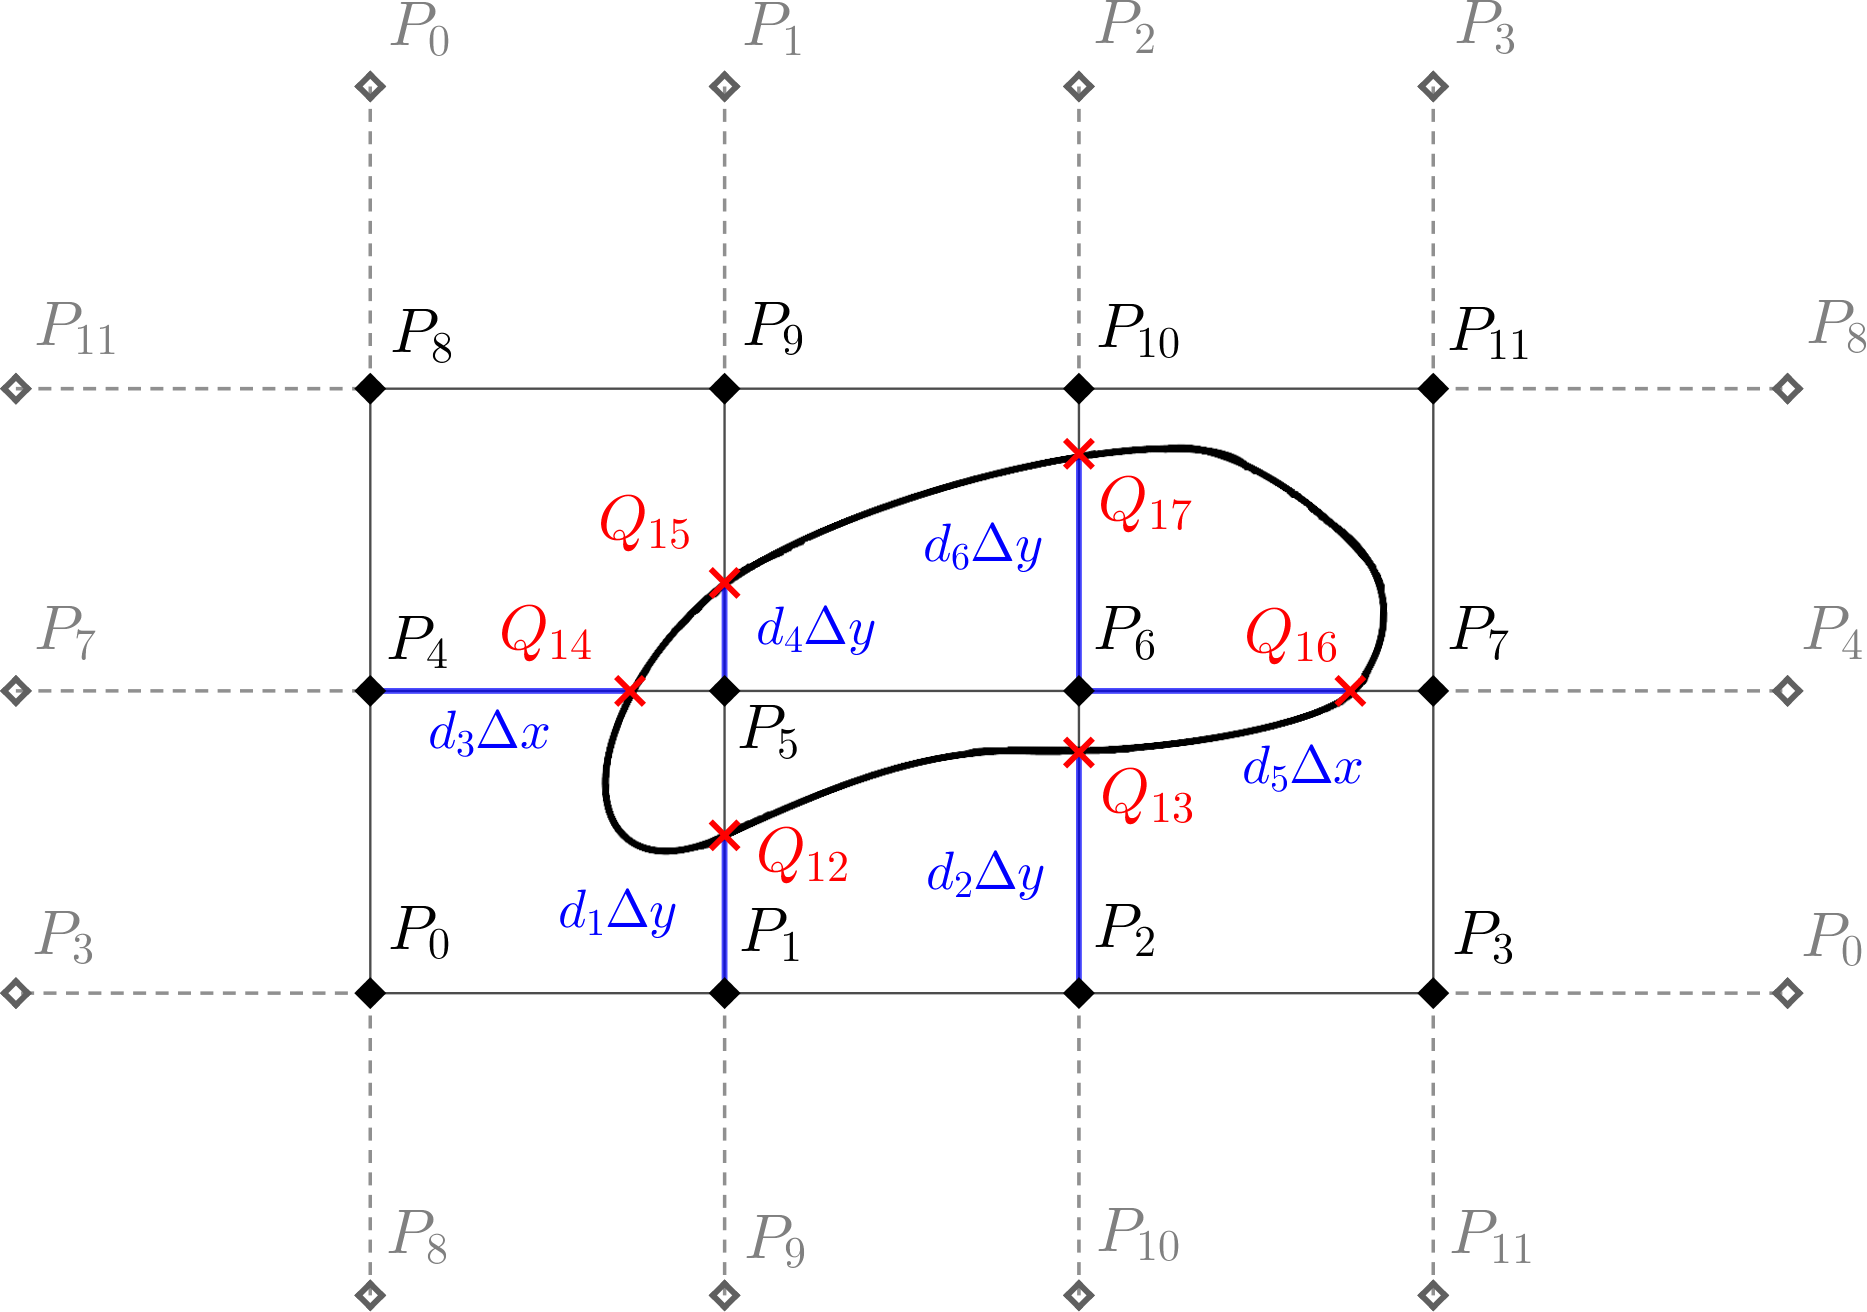
\includegraphics[width=0.6\textwidth]{domain_2d.png}
\end{figure}

\begin{figure}
\centering
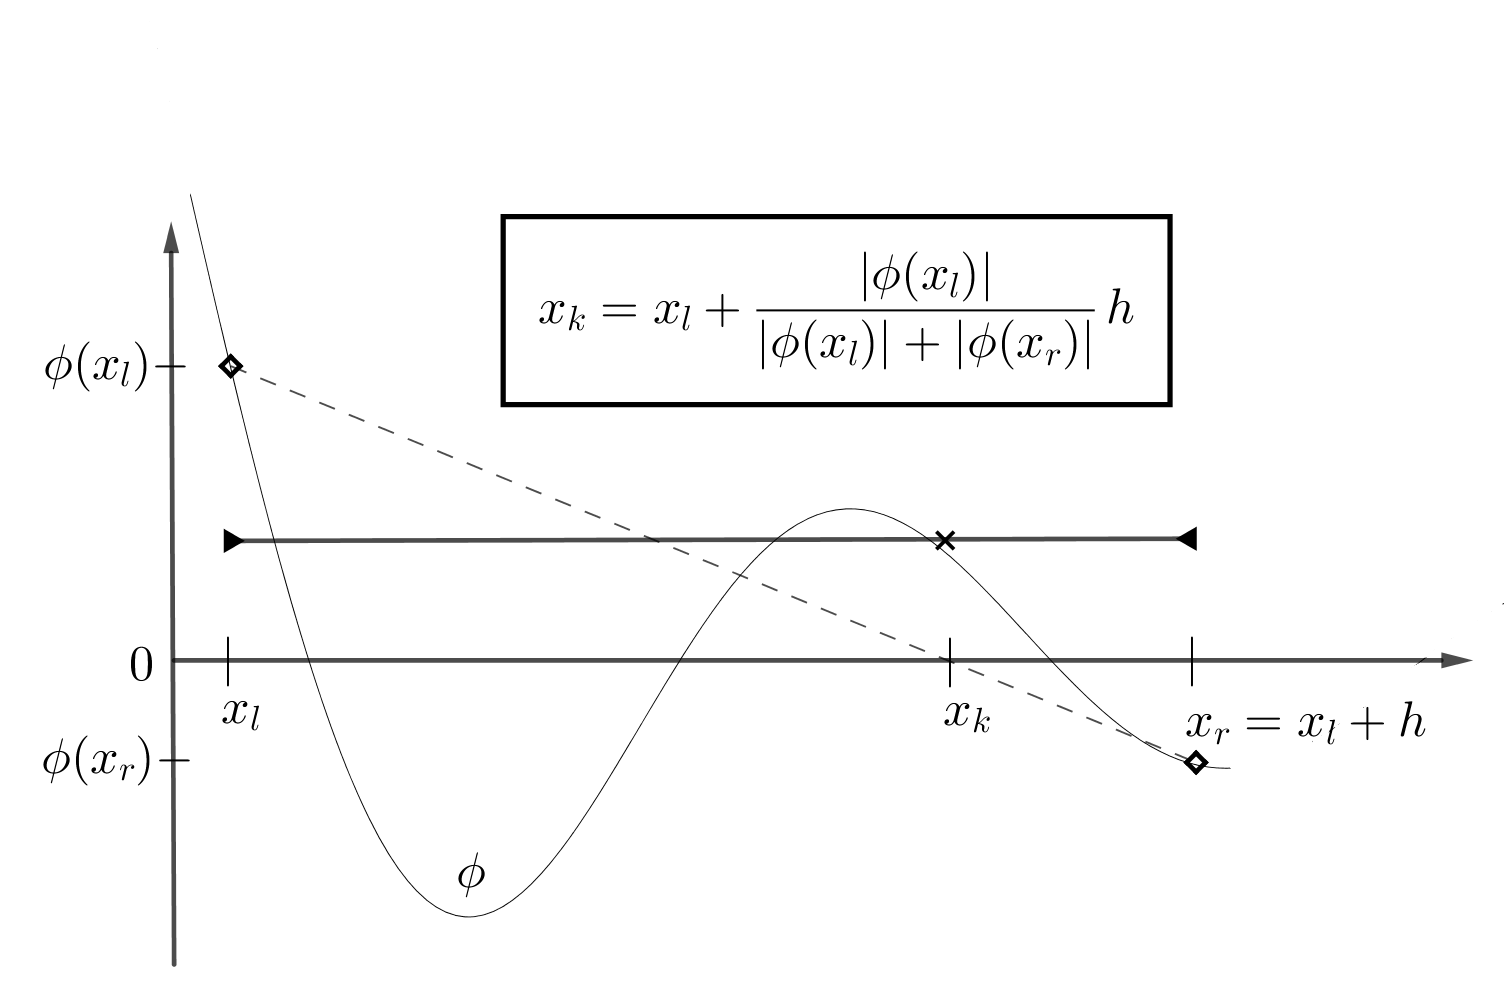
\includegraphics[width=0.6\textwidth]{phi_arete.png}
\end{figure}
\end{document}